\newpage
\section{Destination Tickets}

\subsection{Winning}
\label{sec:winning}
An obvious strategy in \textit{Ticket to Ride} is to collect
Destination Tickets and focus on claiming routes to connect them.
We now investigate the effect of collecting Destination Tickets
on winning the game.
We simulate 10,000 two-player and 10,000 four-player games.
For each Destination Ticket, we calculate the proportion of 
games that the player holding the Destination Ticket won.
Our results appear in \cref{fig:tickets}.
(For example, players in two-player games with Montreal 
to Vancouver won almost $60\%$ of their games.)

\begin{figure}[H]
\centering
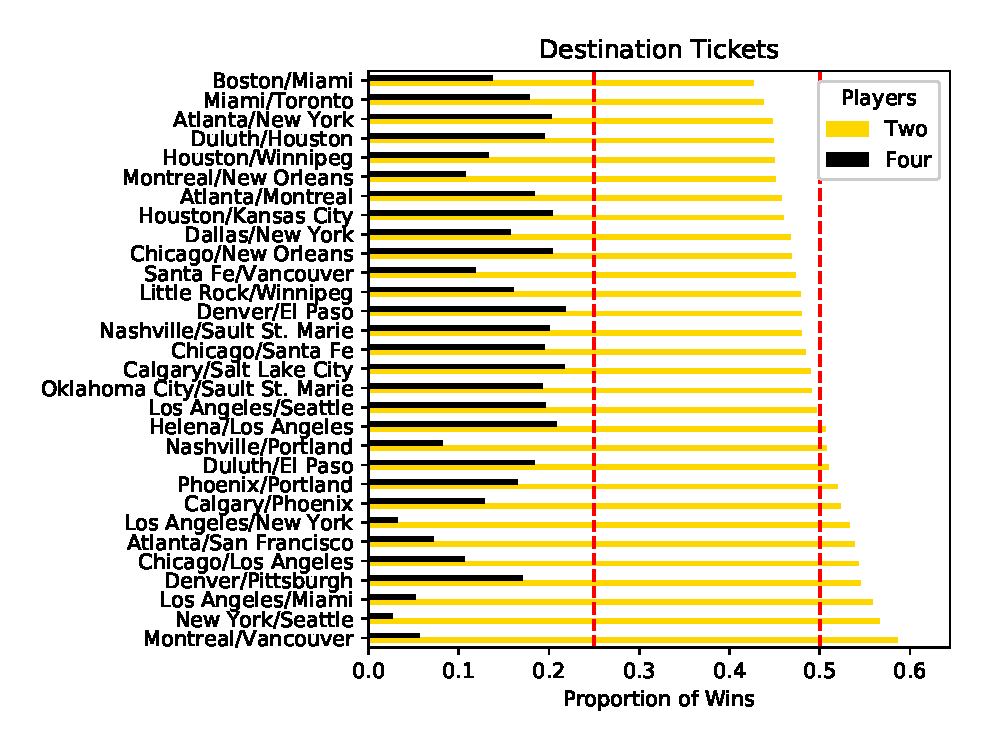
\includegraphics[scale=.6]{figures/destination_tickets}
\caption{For each Destination Ticket,
the proportion of two-player and four-player games that 
the player with the Destination Ticket won.
The vertical red lines at $1/4$ and $1/2$ represent
the expected proportion of games players would win
if Destination Tickets had no effect.}
\label{fig:tickets}
\end{figure}

The vertical red lines at .25 and .5 indicate
the expected proportion of wins if Destination Tickets
had no effect on winning: players in two-player games
would win half the time and players in four-player games
would win a quarter of the time.

In two-player games, there are 13 Destination Tickets 
that win more than the expected $50\%$ of games.
(We say that a Destination Ticket "wins" in the sense
that the player who possesses it wins the game they
are playing.)
In four-player games, there are only eight Destination Tickets
that clearly win more than the expected $25\%$ of games plus
another four on the borderline.
That is, out of the 30 Destination Tickets, roughly a third
in both two- and four-player games win more than expected.
The implication is that a randomly chosen Destination 
Ticket is not advantageous.
However, a subset of Destination Tickets---approximately the same
set for both two- and four-player games---wins more often than expected.
The ones that win the most are Montreal to Vancouver,
New York to Seattle, and Chicago to Los Angeles.

An inspection of \cref{fig:board} shows that the paths between 
the cities in these three Destination
Tickets include the longest routes on the board.
However, to gain a better understanding of what makes some
Destination Tickets more advantageous than others,
we investigate their characteristics
that most closely correlate with winning.
We begin in the next subsection by developing a measure
of the difficulty of connecting one city to another.

\subsection{Effective Resistance}
\label{sec:resistance}
The \textit{Ticket to Ride} board can be mathematically
interpreted as a graph where cities represent
nodes and routes represent edges.
One of the most powerful and natural measures of connectivity
between two nodes on a graph is effective resistance
\cite{ellens2011effective}.
Imagine that the \textit{Ticket to Ride} board were
a large electrical circuit with a unit current
entering at city $a$ and leaving at city $b$.
Effective resistance indicates
how much work a current needs to exert
to get from $a$ to $b$.
In general, the number of paths and length of routes 
determine the effective resistance:
two cities with fewer paths and longer routes
have a higher effective resistance between them
than two cities with many paths and shorter routes.
We calculate the effective resistance for each 
Destination Ticket in order to gain insight
into what makes some more advantageous than others.

On a small graph, effective resistance can be calculated
by repeatedly applying the following rules:
Consider two edges with resistances $r_1$ and $r_0$.
If the two edges are in series (edge 1 connects node $i$ to $j$
and edge 2 connects node $j$ to $k$), then the resistance between
$i$ and $k$ is $r_1 + r_2$.
If the two edges are in parallel (both edge 1 and edge 2 connect
node $i$ to $j$), then the resistance between $i$ and $j$
is $(1/r_1 + 1/r_2)^{-1}$.

On a large graph like the \textit{Ticket to Ride}
board, however, we need a more robust strategy.
We use two separate algorithms to find the effective resistance
of Destination Tickets
\cite{ellens2011effective, wu2004theory}.
Both algorithms calculate the effective resistance by finding 
the eigenvalues of the Laplacian matrix for a given graph.
(The Laplacian is the degree matrix $D$ minus the adjacency
matrix $A$ where $D_{i,i}$ is the weighted degree of node $i$
and $A_{i,j}$ is the resistance of the edges between nodes
$i$ and $j$.)

We let the weight between two cities be the length
of the route connecting them.
In the case that there are two routes between cities,
we let the weight be $(1/r + 1/r)^{-1}=r/2$ where
$r$ is the length of each route.
(There are at most two routes between any two cities
on the \textit{Ticket to Ride} board 
in \cref{fig:board}.)

In the next subsection, we calculate the effective
resistance of all Destination Tickets as a tool
to find what most closely correlates with winning.

\subsection{Winning \& Effective Resistance}
\label{sec:winning_and_resistance}

Our goal is to identify why certain Destination
Tickets win more than others.
We plot Destination Tickets in \cref{fig:resistance}
by the difficulty of connecting their cities (effective
resistance) against their reward.
The line of best fit gives the predicted reward
as a function of difficulty.
We would predict, for example, that the reward for 
connecting the cities
in a Destination Ticket with effective resistance .4 would
be 12 points.
However, completing the $2^\text{nd}$ Destination Ticket 
Houston/Kansas City earns 5 points whereas
completing the $30^\text{th}$ Destination Ticket
New York/Seattle earns 22 points even though
both have resistance approximately .4.
We conclude that Houston/Kansas City is very undesirable
and New York/Seattle is very desirable.
Coloring by the difference from the expected proportion
of wins confirms our conclusion:
Houston/Kansas City has value -.08 (winning $42\%$ of
two-player and $17\%$ of four-player games) while
New York/Seattle has value .09 (winning $59\%$ of
two-player and $34\%$ of four-player games).

Let a Destination Ticket's residual be the difference
between its predicted reward and actual reward.
For the same difficulty, a Destination Ticket
with a high residual has a greater reward
than one with a low residual.
Clearly, the residuals of their Destination Tickets
should affect whether players win: greater point values
increase the number of points relative to the expended
resources.

We compare how well residual 

\begin{figure}[h]
    \centering
    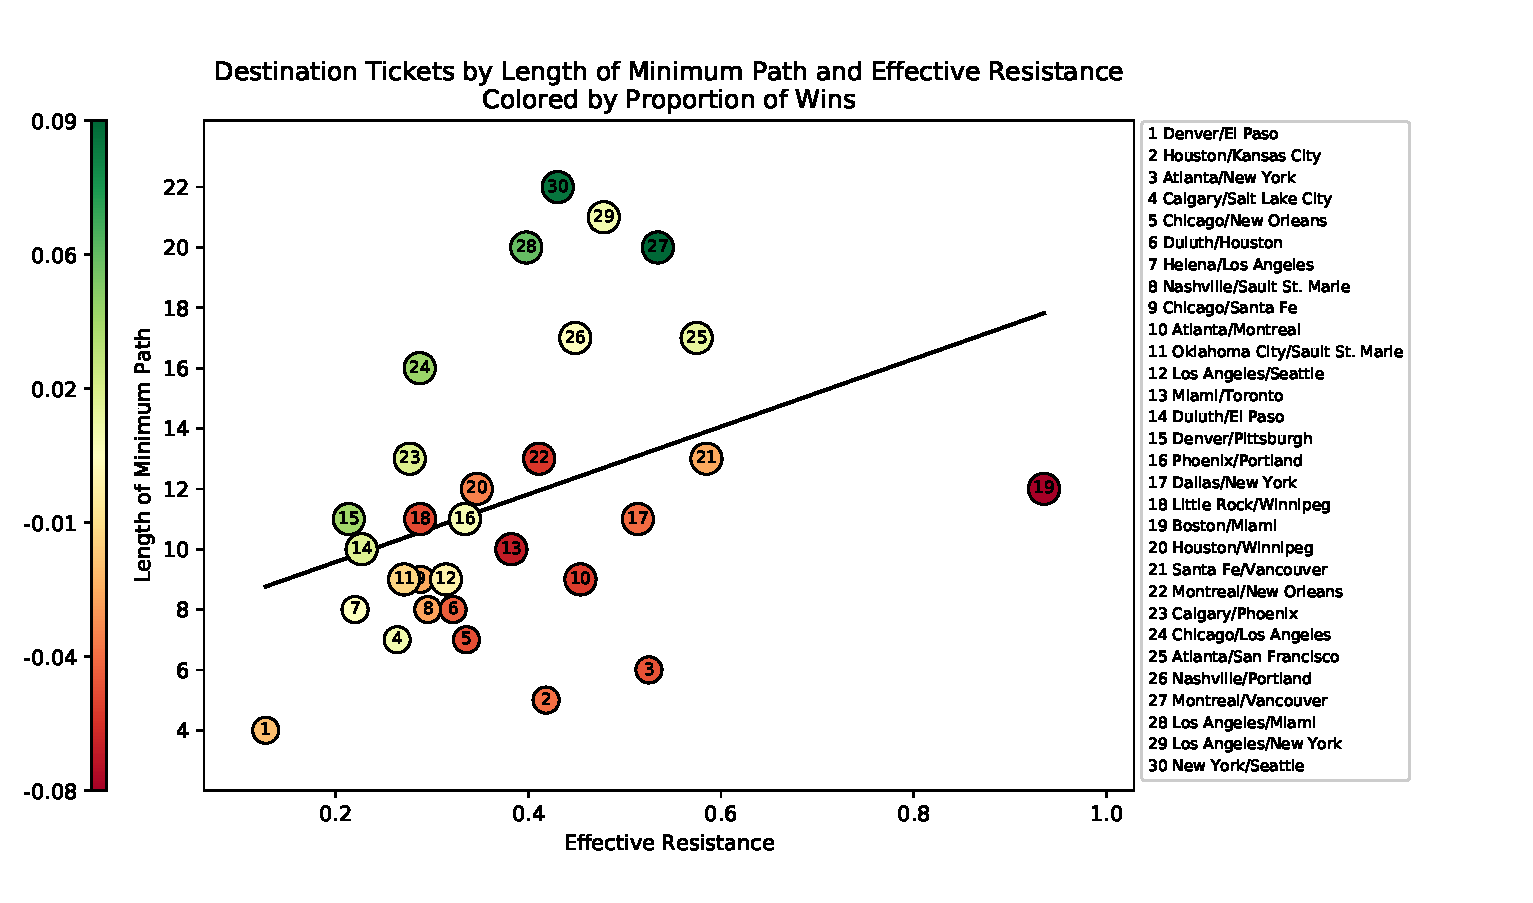
\includegraphics[scale=.6]{figures/resistance_aggregate}
    \caption{Destination Tickets plotted by the
    difficulty of connecting their cities and the reward.
    The line of best fit predicts the value of a Destination
    Ticket based on how challenging its cities
    are to connect.
    Note: the $9^{\text{th}}$ Destination Ticket 
    is obscured by the $11^{\text{th}}$.}
    \label{fig:resistance}
\end{figure}

\begin{figure}[H]
    \centering
    \begin{subfigure}[t]{0.5\textwidth}
        \centering
        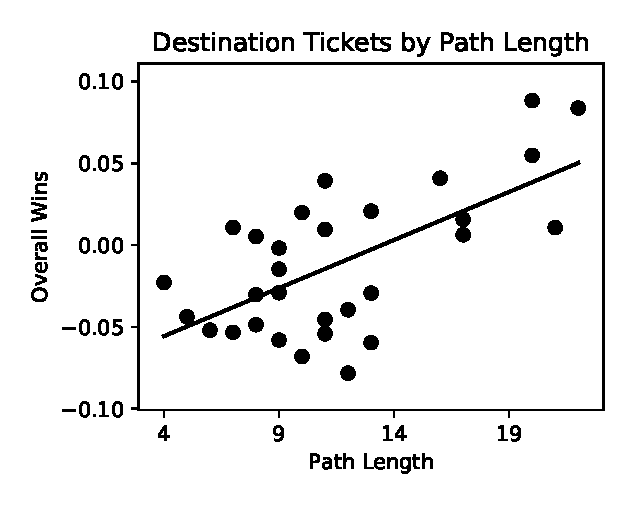
\includegraphics[height=2in]{figures/correlation0}
    \end{subfigure}%
    ~ 
    \begin{subfigure}[t]{0.5\textwidth}
        \centering
        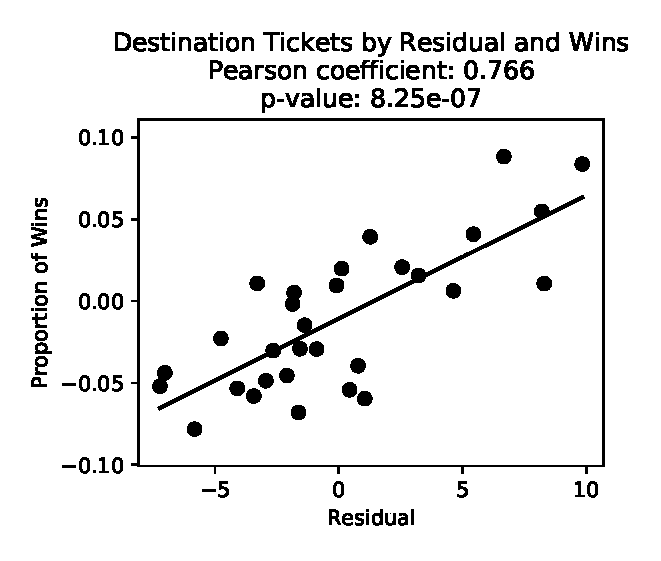
\includegraphics[height=2in]{figures/correlation2}
    \end{subfigure}%
    \caption{Destination Tickets by the proportion of wins
    and path length and residual, respectively.
    The Pearson p-values imply that residual
    correlates more closely with winning than
    path length.}
    \label{fig:correlation}
\end{figure}

\begin{figure}[H]
    \centering
    \begin{subfigure}[t]{0.5\textwidth}
        \centering
        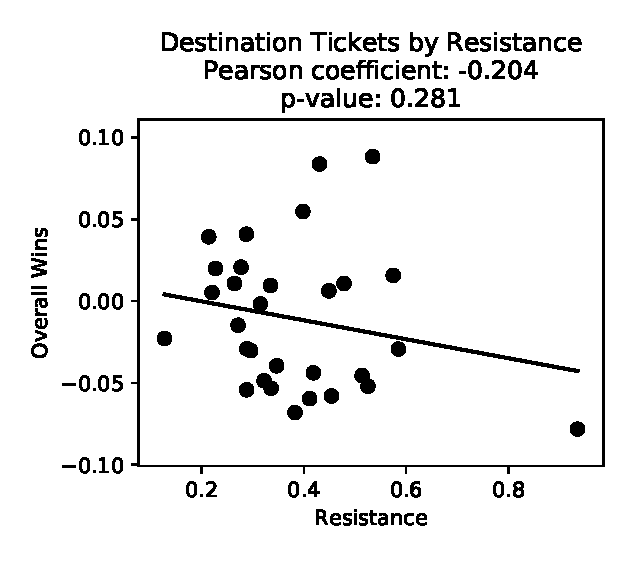
\includegraphics[height=2in]{figures/correlation1}
    \end{subfigure}%
    ~ 
    \begin{subfigure}[t]{0.5\textwidth}
        \centering
        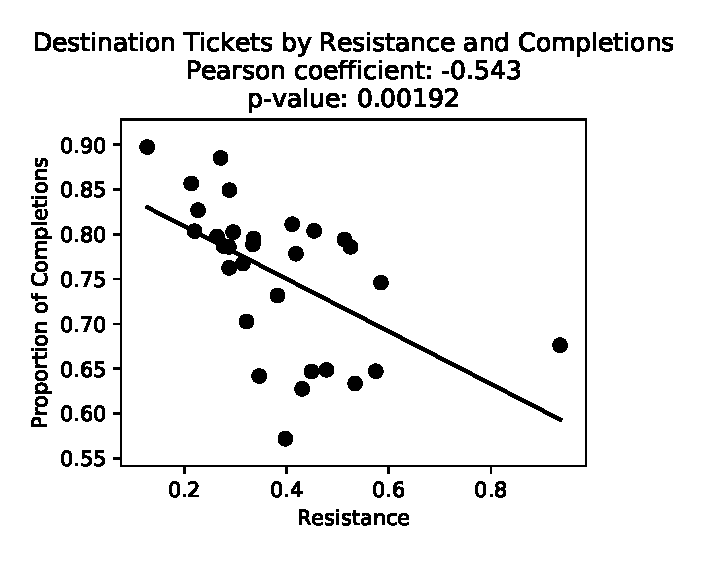
\includegraphics[height=2in]{figures/completion}
    \end{subfigure}%
    \caption{Destination Tickets by the resistance and
    proportion of wins and completions, respectively.
    While it does not correlate well with
    winning, resistance is closely related to
    whether a Destination Ticket gets completed.
    }
    \label{fig:completion}
\end{figure}

\begin{figure}[H]
    \centering
    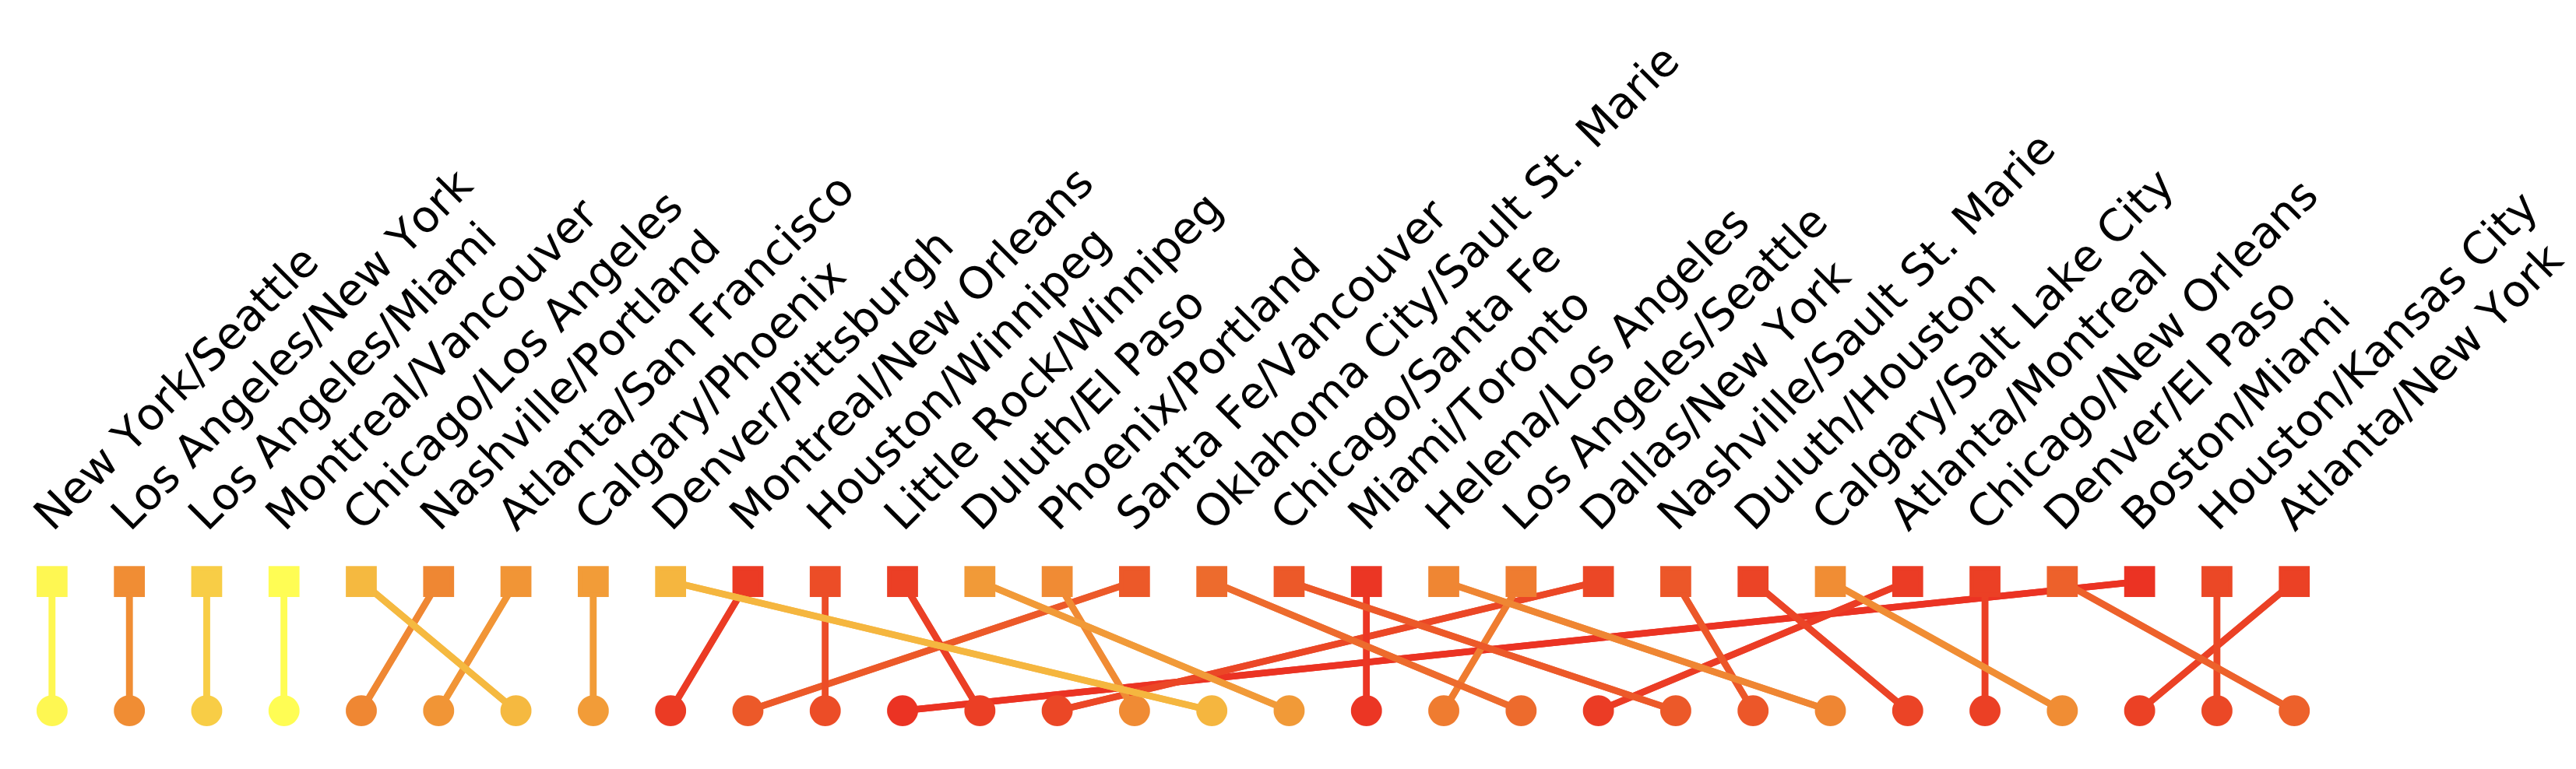
\includegraphics[scale=.25]{figures/rankings2.png}
    \caption{Destination Tickets ordered by path length
    in the bottom row (circles) and by residual
    in the top row (squares). The color
    corresponds to the proportion of overall wins (scale
    from \cref{fig:resistance}).
    Lines indicate the change in rank between
    the two orderings.}
    \label{fig:rankings}
\end{figure}

